\section{Circuit Model of Quantum Computation}
\label{Section:GateModelQC}

The circuit or gate-based model of quantum computation is the most widely studied
framework and the foundation of many quantum algorithms, including Shor's and Grover's
algorithms. In this model, computation proceeds through the application of a sequence
of unitary gates, which evolve the state of the qubits in a discrete, step-wise fashion.

Mathematically, a quantum circuit implements a unitary transformation U on the initial
quantum state, typically chosen as $\ket{0}^{\otimes n}$. This transformation is
decomposed into a series of quantum gates from a universal set of gates. Measurement in
the computational basis is performed at the end of the circuit to extract classical
information from the quantum circuit.

Universality is a crucial property of this model, as it ensures that any unitary transformation --and
therefore any quantum algorithm-- can be implemented using only a finite set of gates. This makes the
circuit model a general-purpose framework, capable of simulating any other model of quantum computation.

Gate-based quantum computation aligns well with digital control paradigms, and most
existing quantum hardware platforms, such as superconducting qubits and trapped ions, are
designed to implement this model. However, the depth and width of circuits that can be
reliably executed on near-term devices are limited by noise, decoherence, and imperfect
gate fidelities.

\begin{figure}[h]
    \centering
    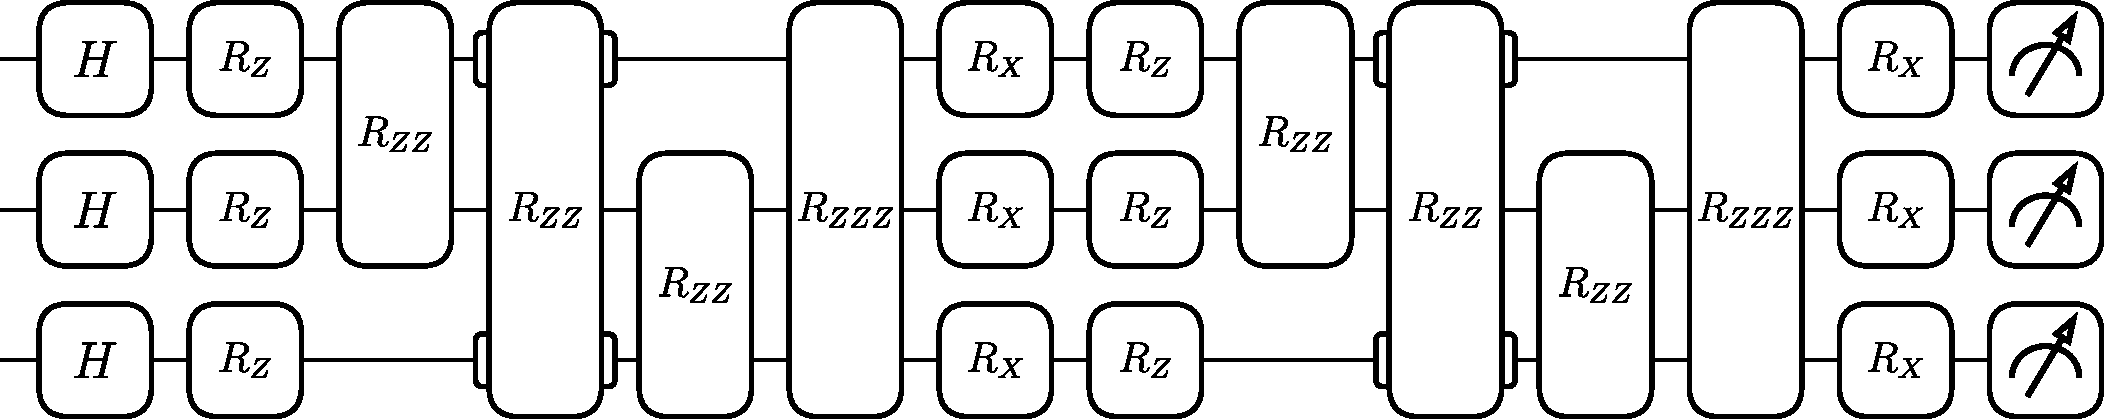
\includegraphics[width=0.9\textwidth]{01-introduction/figs/example_circuit.pdf}
    \caption{Example of a quantum circuit, part of a QAOA protocol that implements integer factorization for a small number.}
    \label{fig:example_circuit}
\end{figure}